\chapter{Methodology}%
\label{chapter:methodology}

\begin{introduction}
In this chapter, i will present the non functional requirements of the applications, as well as the use cases of the user that will interact with them. 
\end{introduction} 




\section{Applications Requirements} 


To identify the requirements of the application, i used the FURPS model. 
The non functional requirements are listed below:

\begin{itemize}
  \item Scalability – The system should be able to handle 500 users simultaneously without degradading the performance.
  \item Reliability – The system should have a high availability of 99\% and the system also should not take longer then 4 hours to recover from a failure.
  \item Performance – The system should not take longer then 2 seconds to respond.
  \item Usability – The train of a new user should not take longer then 8 hours.
  \item Supportability – The system should be suported on the web browsers Chrome, Firefox, Microsoft Edge and Safari.
\end{itemize}

For the functional requirements of the applications, i developed a set of use cases for each user.
The structure of the dealership application was based on the work of the author ~\citet{Setting_the_after_sale_process} and is separated into 4 key user roles: receptionist, mechanic, warehouse operator and administrator.

The receptionist will be responsable to interact with the client, this includes the vehicle check-in and check-out and user comunication in the case of changes in the Initial stablished price and vehicle actions. 
The Use cases of the receptionist are:

\begin{itemize}
    \item Use Case 1.1 – Vehicle Reception
    \begin{itemize}
      \item Scenario – Client arrives at the dealership with a vehicle to be repaired.
      \item Objective – Create a new maintenance request in the system.
      \item System – The receptionist insert in the a form all the information about the initial maintenance request from the client and vehicle and creates a new maintenance request with the date and budget agreed with the client 
    \end{itemize}
    \item Use Case 1.2 – Vehicle Delivery 
    \begin{itemize}
      \item Scenario – The Receptionist delivered the vehicle to the Client.
      \item Objective – Complete the vehicle maintenance process.
      \item System – Sends a report in a pdf format to the client with the information of the maintenance request and alters the maintenance request status in the system to concluded. 
    \end{itemize}
    \item Use Case 1.3 – Collect information about a maintenance request
    \begin{itemize}
      \item Scenario – A Client call the dealership to ask about the maintenance of his vehicle.
      \item Objective – Visualize the maintenance information.
      \item System –  The Receptionist searches a list of maintenance requests by vehicle/customer name/maintenance ID and, by clicking on the element details button, he can view the maintenance details.
    \end{itemize}
    \item Use Case 1.4 – Asking for customer permission
    \begin{itemize}
      \item Scenario – O problem in a vehicle maintenance has occurred and the Initial agreement with client may be broken.
      \item Objective – Inform the client of the problem and achieve an agreement.
      \item System – The Receptionist receives an alert that there has been a change in the initial maintenance budget for a vehicle and/or a change in the maintenance completion deadline, so he needs to contact the customer to inform him. Depending on customer feedback, the receptionist accepts the request, declines the request or terminates the maintenance.
    \end{itemize}
  \end{itemize}  
  \hfill \break


  The mechanic will be responsable to do the maintenance in the vehicle, like oil change, tire change, trade vehicle parts, etc. 
  It will previously evaluate the vehicle, to assure the Initial evaluation of the receptionist is not lacking, and after the maintenance is done, it will write a report of the operations done. 
  The Mechanic Use cases are:

  \begin{itemize}
    \item Use Case 2.1 – View to-do list
    \begin{itemize}
      \item Scenario – The mechanic arrives at dealership and wants to see what tasks he has to do today.
      \item Objective – See the day's work organization.
      \item System – The mechanic watches a list of tasks that were assign from the administrator, as soon as he enters the system. Each task is accompany by a description, a priority, the vehicle identification, a set of actions to be performed and comments from other users. 
    \end{itemize}
    \item Use Case 2.2 – Carry out a vehicle analysis 
    \begin{itemize}
      \item Scenario – A new vehicle needs to be analyzed.
      \item Objective – Confirm the Initial analysis of the receptionist and search for additional problems.
      \item System – The mechanic enters the problems he finds in the vehicle into the system. 
    \end{itemize}
    \item Use Case 2.3 – Prepare a list of necessary parts
    \begin{itemize}
      \item Scenario – After vehicle analysis.
      \item Objective – Elaborate a request of vehicle parts for the warehouse.
      \item System – The mechanic selects the parts of the vehicle that need to be replaced and sends a request with the new parts to the warehouse.
    \end{itemize}
    \item Use Case 2.4 – Collect the requested parts in the Warehouse
    \begin{itemize}
      \item Scenario – The mechanic goes to the warehouse to collect new parts for the vehicle.
      \item Objective – Collect parts to replace the damaged parts in the vehicle.
      \item System – The mechanic add the new parts to the vehicle in the system.
    \end{itemize}
    \item Use Case 2.5 – Deliver damaged parts to the Warehouse
    \begin{itemize}
      \item Scenario – The mechanic goes to the warehouse to deliver the damaged parts.
      \item Objective – Register the parts as being damaged.
      \item System – The mechanic removes the damaged parts from the vehicle and change the status to damaged.
    \end{itemize}
\item Use Case 2.6 – Vehicle maintenance
\begin{itemize}
  \item Scenario – A new vehicle is ready for a maintenance.
  \item Objective – The mechanic will do the vehicle maintenance (oil change, tire change, vehicle wash…).
  \item System – The mechanic sees a set of tasks that he needs to do to complete the vehicle maintenance and whenever he finishes a task, he marks it as completed.
\end{itemize}
\item Use Case 2.7 – Making the repair report
\begin{itemize}
  \item Scenario – After vehicle maintenance.
  \item Objective – Conclude the maintenance of a vehicle.
  \item System – The Mechanic enters into the system all operations and tests carried out on the system as well as their results.
\end{itemize}
\end{itemize}
\hfill \break

The warehouse operator is responsable to manage the dealer's stock and ask for suplies, so i write the following use cases:

\begin{itemize}
  \item Use Case 3.1 – View the different parts that the warehouse possess
  \begin{itemize}
    \item Scenario – The warehouse worker wants to view the quantity of a certain parts that the warehouse possess.
    \item Objective – Show quantitative warehouse information.
    \item System – List of all parts and their quantities that the warehouse possess. 
  \end{itemize}
  \item Use Case 3.2 – Requesting purchasing service 
  \begin{itemize}
    \item Scenario – The warehouse worker discovers that he has an insufficient number of parts for maintenance or anticipates that this part will be missing soon.
    \item Objective – Request permission to purchase parts from the supplier.
    \item System – The Warehouse Worker will place a purchase order for parts. The system notifies the administrator via the platform and by email requesting authorization to do the purchase. 
  \end{itemize}
  \item Use Case 3.3 – Registration of new parts in the System
  \begin{itemize}
    \item Scenario – The warehouse purchased several parts from a supplier.
    \item Objective – Register new parts in the system.
    \item System – Warehouse operator adds a specific type of part to the system with its appropriate description and identification.
  \end{itemize}
\end{itemize}
\hfill \break

The last user of the application is the administrator or Workshop Manager. This user is in charge of managing the platform and the dealership. So the main use cases I encountered are:

\begin{itemize}
  \item Use Case 4.1 – Authorizing purchases
  \begin{itemize}
    \item Scenario –  The administrator received a purchase request.
    \item Objective – Authorize or reject a purchase authorization request.
    \item System – List of all purchase authorization requests, as well as their details. The administrator can change the status of this request, rejecting or authorizing. 
  \end{itemize}
  \item Use Case 4.2 – View history of maintenance performed
  \begin{itemize}
    \item Scenario – The administrator wants to gather information from recently performed maintenance.
    \item Objective – View information about a specific maintenance that occurred.
    \item System – List of all maintenance that occurred as well as its details (who carried it out, which parts were removed, the name of the customer, tests carried out and their results…). 
  \end{itemize}
  \item Use Case 4.3 – Develop statistics
  \begin{itemize}
    \item Scenario – The administrator wants to gather statistics on maintenance that was carried out in the last month.
    \item Objective – View information about maintenance over a given period of time.
    \item System – Presentation of the number of parts replaced, number of purchases, total price spent on new parts, remuneration for maintenance, average customer's rating, etc.
  \end{itemize}
  \item Use Case 4.4 – Assign roles to employees
  \begin{itemize}
    \item Scenario – A new employee has been hired.
    \item Objective –  Assign roles to new employee.
    \item System – The administrator assigns the new employee a certain role and set of permissions.
  \end{itemize}
  \item Use Case 4.5 – Assign tasks to the employees
  \begin{itemize}
    \item Scenario – A new maintenance request has been requested.
    \item Objective – Assign and organize tasks to different employees.
    \item System – The administrator assigns the various stages of vehicle maintenance to the various workshop employees.
  \end{itemize}
\end{itemize}
\hfill \break

The client application will only be interacted by a role of users, the client.
The use cases are listed below:

\begin{itemize}
  \item Use Case 5.1 – View current maintenance status
  \begin{itemize}
    \item Scenario – The Customer wants to find information regarding the vehicle maintenance procedure.
    \item Objective – Display current maintenance status.
    \item System – The system will illustrate all the maintenance steps that the vehicle has already undergone, as well as those that remain to be completed. 
  \end{itemize}
  \item Use Case 5.2 – Notify the customer of the end of maintenance 
  \begin{itemize}
    \item Scenario – Vehicle maintenance has been completed and the customer can now collect the vehicle.
    \item Objective – Notify the user of the end of maintenance.
    \item System – The system will show a native notification on the customer's cell phone informing that the vehicle is ready to be picked up. 
  \end{itemize}
  \item Use Case 5.3 – Rating of the service provided
  \begin{itemize}
    \item Scenario – The client receives the vehicle and the receptionist completes the maintenance process.
    \item Objective – Get feedback from the client.
    \item System – The system will show a form to the client asking about service provided. The crucial points are time of the service, service quality, user interaction and price.
  \end{itemize}
\end{itemize}
\hfill \break

With this requirements, both application should increase the efficiency of the work at the dealership and improve client loyalty to ensure profit.


\section{Applications Workflow}

After the development of the use cases i designed a flow chart to understand the users' interaction with the system and each other. The chart is visible in figure \ref{fig:figure2}.

\begin{figure}[h]
  \caption{Use Case Flow Chart of the Client, Receptionist, Mechanic, Warehouse Operator and administrator.}
  \centering
  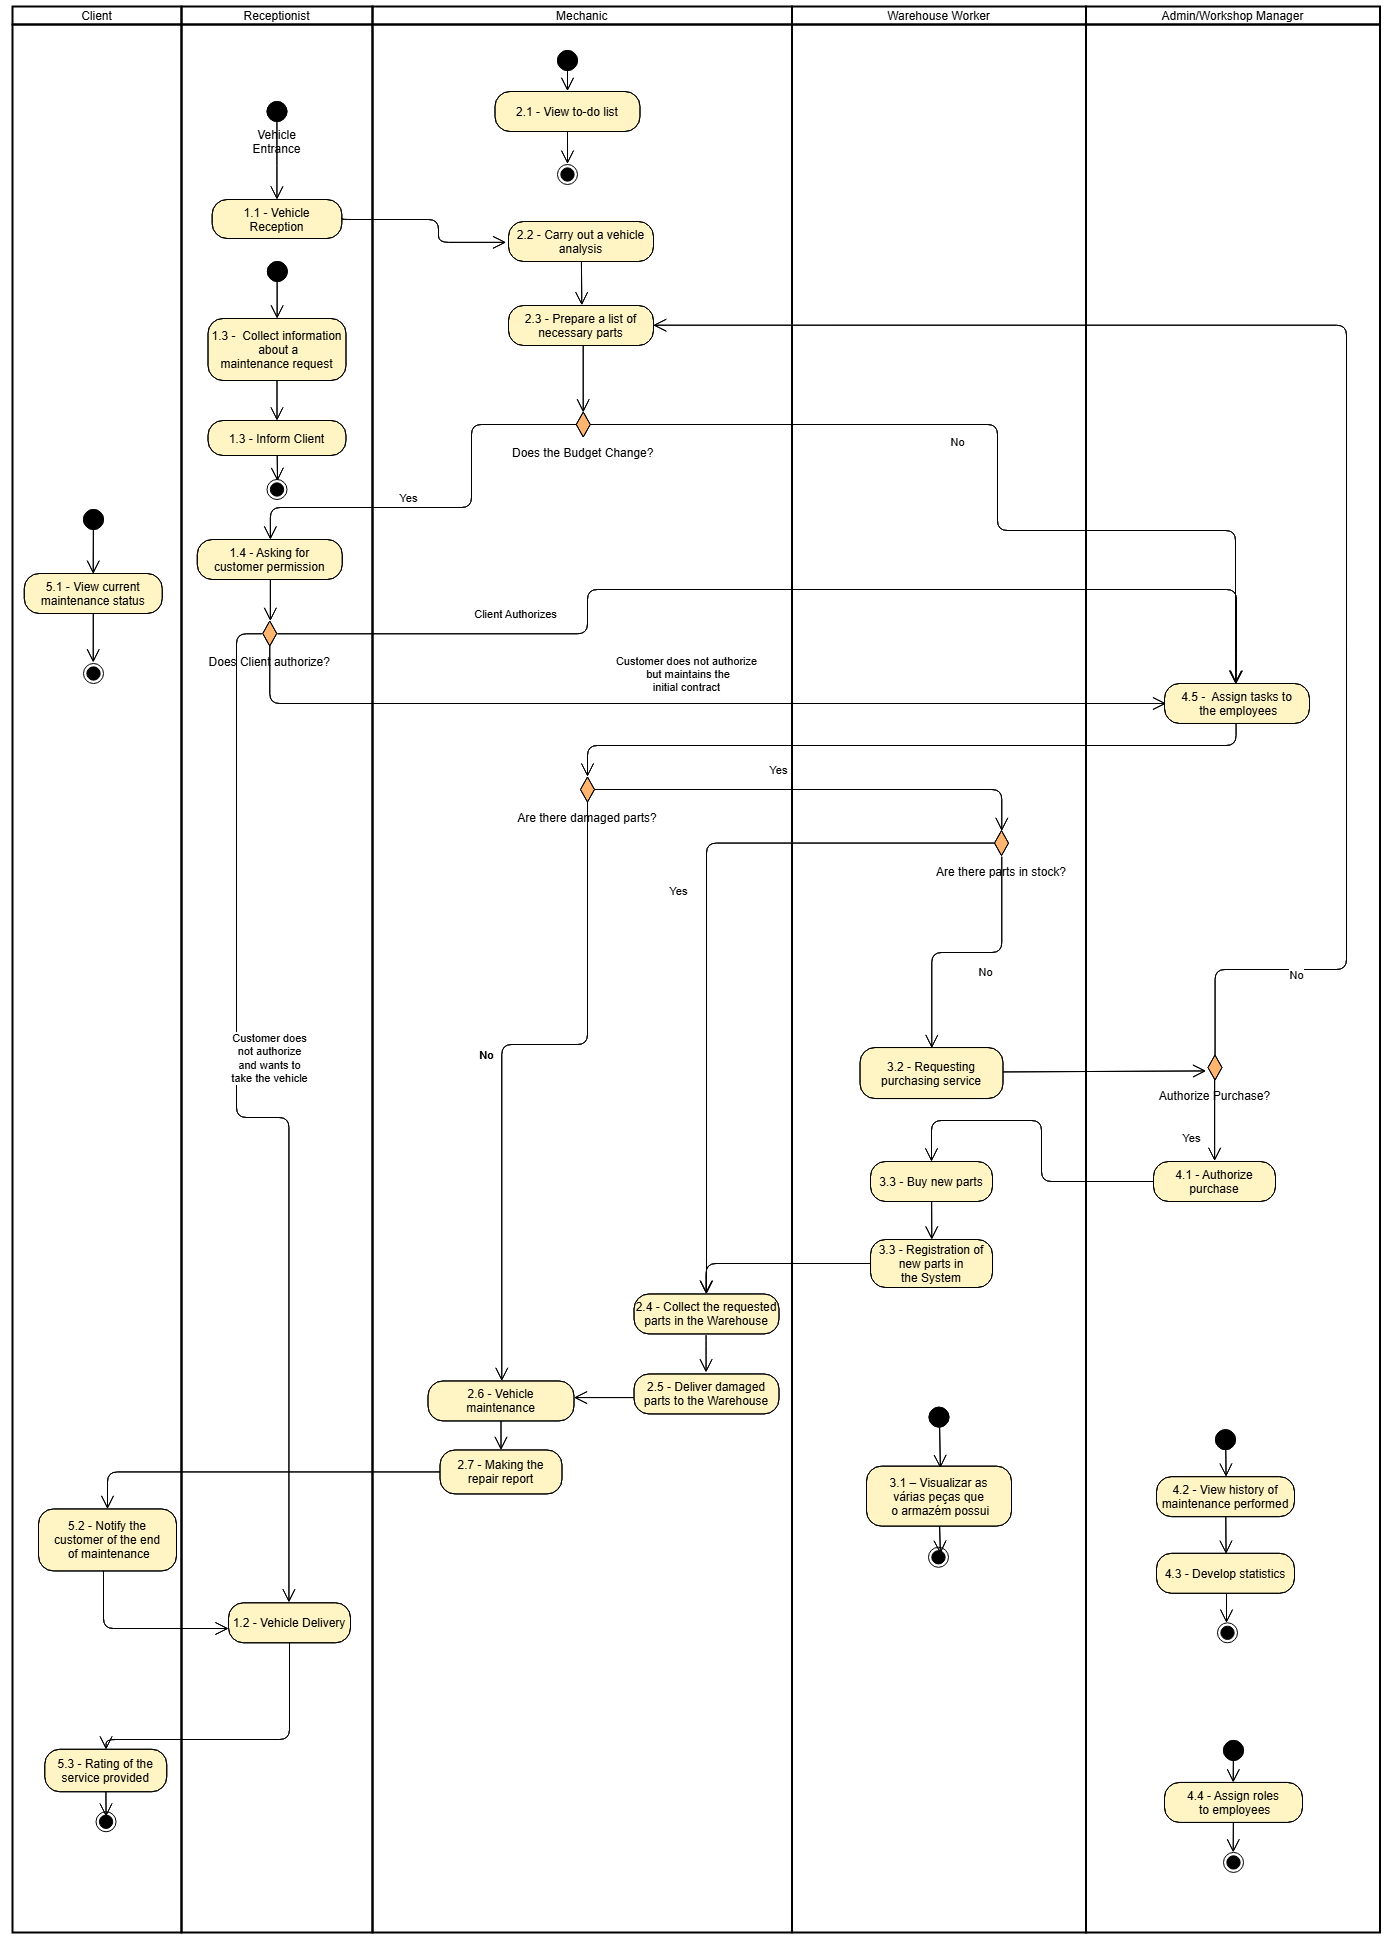
\includegraphics[width=\textwidth]{figs/UseCaseDiagram}
  \label{fig:figure2}
\end{figure}

The system main flow starts when a Client arrives at the dealership for a vehicle maintenance. 
The receptionist get some inputs from the client and decides a Initial budget and check-out date agreed with the Client and insert the information in the system (Use Case 1.1).
After that, a worker will be responsable to the analysis of the vehicle. 
He will add to the system all the problem he finds and the necessary parts that need to be replaced (Use Case 2.2 and 2.3).


If the budget to complete the work or the expected time changes, an alert is sent to the receptionist to inform the Client (Use Case 1.4). 
The result of this interaction must be authorize the changes and continue the work; not authorize the changes but continue as Initially agreed; and 
In the case of the Client not authorizing the changes and wanting to check out the vehicle, the vehicle is delivery and the app will request the client to rate the service (Use Case 1.2 and 5.3). 
If the client does not authorize the changes but wants the maintenance to continue as Initially agreed, the maintenance process continues as if the client authorizing the changes. 
The maintenance process information would only be alterated.
The admin will receive a notification of the new tasks and will assign them to each worker (Use Case 4.5).

From there on, the maintenance process can or can not require the need to a vehicle part to be replaced. 
In the negative case the vehicle goes to the responsable mechanic to do the oil change, tire change, wash, etc (Use Case 2.6). 
In the affirmative case, the Warehouse Operator will check if the parts the mechanic request are available in stock. 
If it does, the operator accepts the request and delivers the parts to the mechanic, which will replace the parts of the vehicle, add it to the system, deliver the damaged parts to the warehouse and do the maintenance (Use Case 2.4, 2.5 and 2.6). 
If it does not, the operator need to buy new parts from the supplier, so he iniciates a new requesting purchase that can be authorized by the admin. 
In the optimal case, the admin accepts the purchase, the operator buy the new parts, register them in the system and delivers them to the mechanic. 
In the worst scenario, the admin reject the purchase and the mechanic needs to request new parts and restart the process (Use Case 2.3).    

Finally, when the vehicle maintenance is finished, the mechanic inserts into the system all operations and tests carried out as well as their results (Use Case 2.7). 
The system notifies the customer that the vehicle is ready for the check out and, when the receptionist delivers the vehicle to the Customer, the client application ask for the client to rate the system (Use Case 5.2, 1.2 and 5.3).

There are also afew secondary flows visible in the figure \ref{fig:figure2}. 
This flows are listed below:
\begin{itemize}
  \item The client enters the aplication to check the status of the maintenance (Use case 5.1);
  \item The mechanic enters the application to view the task he has to do (Use Case 2.1); 
  \item The Warehouse Operator enters the aplication to visualize the diverse parts and components in the warehouse (Use case 3.1); 
  \item The Admin enters the application to assign roles and/or permission to the employees (Use Case 4.4); 
  \item The Admin enters the application to gather information about a maintenance performed and see statistics about tha information (Use Case 4.2 and 4.3); 
\end{itemize}
 








